% -*- root: ../main.tex -*-

\documentclass[../main.tex]{subfiles}
\begin{document}

\chapter{Reduzierte-Basis-Methode} % (fold)
\label{chapter:rbm}

% chapter reduzierte_basis_methode (end)

Nun wird aufbauend auf das Petrov-Galerkin-Verfahren des vorherigen Kapitels die Reduzierte-Basis-Methode eingeführt und auf das gegebene Setting übertragen.
Anschließend wird die numerische Umsetzung dieser für unsere bereits in \cref{sub:grb:gv:numerische_umsetzung} betrachtete Problemstellung angegangen und die Ergebnisse diskutiert.

\section{Grundlagen} % (fold)
\label{sub:grb:rb:grundlagen}

Wir beginnen mit einer kurzen Motivation und Einführung der Reduzierte-Basis-Methoden.
Dabei handelt es sich um ein relativ junges Verfahren, welches besonders in den letzten Jahren viel Aufmerksamkeit und Weiterentwicklung erfahren hat.
Eine weitaus umfassendere Einführung als die nachfolgende findet man beispielsweise in der Arbeit von \textcite{Patera:2007un}.

Um die Idee hinter der Reduzierte-Basis-Methode zu erklären, benötigen wir das folgende Setting: Sei $\mathcal P \subset \mathbb{R}^{p}$ eine abgeschlossene und konvexe Parametermenge und sei das folgende parametrische Variationsproblem gegeben:
Sei $\mu \in \mathcal P$, finde $u(\mu) \in \mathcal X$ mit
\begin{equation}
    \label{eq:rbm_varprob_allgemein}
    b(u(\mu), v; \mu) = f(v; \mu) \quad \fa v \in \mathcal Y,
\end{equation}
wobei $b(\blank, \blank; \mu) \colon \mathcal X \times \mathcal Y \to \mathbb{R}$ eine Bilinearform und $f(\blank; \mu) \colon \mathcal Y \to \mathbb{R}$ ein lineares Funktional ist, so dass für alle $\mu \in \mathcal P$ das obige Variationsproblem korrekt gestellt ist.
Probleme dieser Art werden oft, wie beispielsweise in \autoref{kapitel_petrov_galerkin} beschrieben, mittels Galerkin-Verfahren auf hochdimensionalen Räumen $\mathcal X^{\mathcal N}$ und $\mathcal Y^{\mathcal N}$ gelöst.
Wir stützen uns darauf, dass der Fehler dieser Diskretisierung theoretisch beliebig klein gehalten werden kann und bezeichnen im Folgenden die Räume $\mathcal X^{\mathcal N}$ und $\mathcal Y^{\mathcal N}$ als Truth-Ansatz- respektive Truth-Testraum und die entsprechende diskrete Lösung $u^{\mathcal N}(\mu) \in \mathcal X^{\mathcal N}$ als Truth-Lösung.

Unter der Annahme, dass die Lösung $u(\mu) \in \mathcal X$ eine gewissen Regularität bezüglich des Parameters $\mu \in \mathcal P$ aufweist, hat die durch die Lösungen gebildete Mannigfaltigkeit $\mathcal M^{\mathcal N} = \Set{u^{\mathcal N}(\mu) \in \mathcal X^{\mathcal N} \given \mu \in \mathcal P}$ meist eine eher niedrige Dimension, vergleiche \autoref{fig:figure1}.
Hier setzen die Reduzierte-Basis-Methoden an; der Reduzierte-Basis-Ansatzraum $\mathcal X_{N}$ wird definiert als $N$-dimensionale Approximation
\begin{equation}
    \mathcal X_{N} = \spn\Set{u^{\mathcal N}(\mu_{i}) \given i = 1 \dots N} = \spn\Set{\xi_{1}, \dots, \xi_{N}}
\end{equation}
an $\mathcal M^{\mathcal N}$, wobei $N \ll \mathcal N$ wünschenswert ist.
Die Reduzierte-Basis-Lösung $u_{N}(\mu)$ wird dann durch erneute Galerkin-Projektion von \autoref{eq:rbm_varprob_allgemein} auf $\mathcal X_{N}$ und einen noch näher zu bestimmenden Reduzierte-Basis-Testraum $\mathcal Y_{N}$ bestimmt.

\begin{figure}[tb]
    \centering
    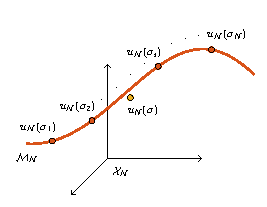
\includegraphics[width=0.6\textwidth]{figures/rb.pdf}
    \caption[%
    Skizzenhafte Darstellung der Funktionsweise der Reduzierte-Basis-Methode.
    ]{
        Skizzenhafte Darstellung der Funktionsweise der Reduzierte-Basis-Methode.
        Die Reduzierte-Basis-Approximation $u_{N}(\mu)$ ergibt sich als Linearkombination der Finite-Elemente-Snapshots $u^{\mathcal N}(\mu_{i})$, welche mutmaßlich eine glatte parametrische Manigfaltigkeit bilden.
        }
    \label{fig:figure1}
\end{figure}

\subsection{Bestimmung der inf-sup-Konstante} % (fold)
\label{sub:bestimmung_der_inf_sup_konstante}

Wie bei der Herleitung des Fehlers zwischen der Reduzierte-Basis-Lösung und der Truth-Lösung ersichtlich wurde, wird eine Möglichkeit benötigt die inf-sup-Konstante $\beta^{\mathcal N}(\mu)$ für viele verschiedene Parameter $\mu \in \mathcal P$ zu bestimmen, oder zumindest von unten zu beschränken.
Hierfür bietet sich die sogenannte \ac{SCM} an, welche speziell für die Anwendung bei Reduzierte-Basis-Methoden entwickelt wurde und eine sinnvolle Offline-Online-Zerlegung ermöglicht.

Wir orientieren uns dabei an dem Originalartikel von \textcite{Huynh2007} und den Verbesserungen von \textcite{Chen2009}.

Seien wie zuvor $\mathcal X^{\mathcal N}$ und $\mathcal Y^{\mathcal N}$ Ansatz- beziehungsweise Testraum des Truth-Variationsproblems welches durch
\begin{equation}
0
\end{equation}


% subsection bestimmung_der_inf_sup_konstante (end)

% subsection grundlagen (end)

\section{Numerische Umsetzung} % (fold)
\label{sub:grb:rb:numerische_umsetzung}

% subsection numerische_umsetzung (end)

% section reduzierte_basis_methode (end)

% chapter reduzierte_basis_methode (end)

\end{document}
